\section{Basic Descriptive Techniques}

Statistical techniques for analyzing time series vary from relatively straightforward descriptive techniques to sophisticated inferential techniques. This chapters introduces the former. Descriptive techniques should be tried before attempting more complicated procedures, because they are important in `cleaning' the data, and then getting a `feel' for them, before trying to generate ideas as regards to a suitable model.

This chapter focuses on ways of understanding typical time-series effects, such as trend, seasonality, and correlations betyween successive observations.



% ----------2.1----------
\subsection{Types of Variation}
Traditional methods of time-series analysis are mainly concerned with decomposing the variation in a series into components representing trend, seasonal variation and other cyclic changes. Any remaining variation is attributed to `irregular' fluctuations. This approach is not always the best but is particularly valuable when the variation is dominated by trend and seasonality. 

\textit{Seasonal variation}
Many time series, such as sales figures and temperature readings, exhibit variation that is annual in period. For example, unemployment is typically `high' in winter but low in summer. This yearly variation is easy to understand, and can readily be estimated if seasonality is of direct interest. Alternatively, seasonal variation can be removed from the data to give deseasonalized data.

\textit{Other cyclic variations}
Apart from seasonal effects, there are some other variations of time series at a fixed period due to some other physical cause. For example, daily variations in temperature depend on what time of the day it is. 

\textit{Trend}
This may be loosely defined as `long-term change in the mean level'. However, this largely depends how we define the term `long-term'. It can be a year to even 50 years depending on the span of the time series.

\textit{Other irregular fluctutations}
After trend and cyclic variations have been removed from a set of data, we are left with residuals that may or may not be `random'. We'll examine later whether this can be explained in terms of probability models, such as the moving average (MA) or autoregressive (AR) models.



% ----------2.2----------
\subsection{Stationary Time Series}
Broadly speaking a time series is said to be stationary if there is no systematic change in mean (no trend), if there is no systematic change in variance and if strictly periodic variations have been removed. In other words, the properties of one section of the data are much like those of any ohter section.

Much of the probability theory of time series is concerned with stationary time series, and for this reason time series analysis often requires one to transform a non-stationary time series to a stationary one so as to use the theory. For example, we can remove the trend and seasonality and model the resuals by a stationary stochastic process. However, sometimes we may be more interested in the non-stationary components too!



% ----------2.3----------
\subsection{The Time Plot}
Ths first, and most important, step in any time-series analysis is to plot the observations against time. This grap, called the time plot, will show up important features of the series such as trend, seasonality, outliers and discontinuities. 

Plotting a time series is not as easy as is sounds. The choice of scales, siz eof intercept, way that points are plotted may substantially affect the way the plot looks. Not all computer software plots the time series well, so we'll have to adjust manually sometimes.



% ----------2.4----------
\subsection{Transformations}
Plotting the data may suggest that it is reasonable to transform them by, for example, taking logs or square roots. The three main reasons for making a transformation are as follows:

\textit{(i) To stabilize the variance}

If there is a trend in the series and the variance appears to increase with the mean, they it may be advisable to transform the data. In particular, if the standard deviation is directly proportional to the mean, a logarithmic transformation is indicated. On the other hand, if the variance changes through time without a trend being present, then a transformation will not help.

\textit{(ii) To make the seasonal effect additive}

If there is a trend in the series and the size of the seasonal effect appears to increase with the mean, then it may be advisable to transform the data so as to make the seasonal effect constant from year to year. The seasonal effect is then said to be additive. In particular, if the size of the seasonal effect is directly proportional to the mean, then the seasonal effect is said to be multiplicative and a logarithmic transformation is appropriate to make the effect additive. However, this transformation will only stabilize the variance if the error term is also thought to be multiplicative (see Section 2.6), a point that is sometimes overlooked.

\textit{(iii) To make the data normally distributed}

Model building and forecasting are usually carried out on the assumption that the data are normally distributed. In practice this is not necessarily the case; there may, for example, be evidence of skewness in that there tend to be `spikes' in the time plot that are all in the same direction (either up or down). This effect can be diffcult to eliminate with a transformation and it may be necessary to model the data using a different ‘error’ distribution.

The logarithmic and square root transformations above are special cases of a general class of transformations called the Box-Cox transformation. Given an observed time series $\{ x_t \}$ and a transformation parameter $\lambda$, the transformed series is given by 
\[ y_t = \begin{cases}
	(x_t^\lambda - 1) / \lambda &\text{ if } \lambda \neq 0, \\
	\log_{}{(x_t)} &\text{ if } \lambda = 0.
\end{cases}
\]
The best value of $\lambda$ is usually `guesstimated'. 

However, Nelson and Granger (1979) found that there is little
improvement in forecast performance when a general Box–Cox transformation
was tried on a number of series. There are cases where the transformation fails to stabilize the variance. Usually, transformations should be avoided wherever possible
except where the transformed variable has a direct physical interpretation.
For example, when percentage increases are of interest, then taking logarithms
makes sense.




% ----------2.5----------
\subsection{Analyzing Series that Contain a Trend and No Seasonal Variation}
The simplest type of trend is the familiar `linear trend + noise', for which the observation at time $t$ is a random variable $X_t$ given by 
\[ X_t = \alpha + \beta t + \varepsilon_t, \]
where $\alpha, \beta$ are constants and $\varepsilon_t$ denotes a random error term with zero mean. The mean level at time $t$ is given by $m_t = \alpha + \beta t$; which is some times called the `trend term'. However, some authors denote $\beta$ as the trend so it depends on the context.

The trend above is a deterministic function of time and is
sometimes called a global linear trend. In practice, this generally provides
an unrealistic model, and nowadays there is more emphasis on models that
allow for local linear trends. One possibility is to fit a piecewise linear
model where the trend line is locally linear but with change points where the
slope and intercept change (abruptly). We can also assume that $\alpha, \beta$ evolve stochastically, giving rise to a stochastic trend.

Now we describe some methods to describing the trend.


\subsubsection{Curve Fitting}
A traditional method of dealing with non-seasonal data with a trend is to fit a simple function such as a polynomial, a Gompertz curve, or a logistic curve. The Gompertz curve can be written in the form
\[ \log_{}{x_t} = a + br^t \]
where $a, b, r$ are parameters with $0 < r < 1$, or in the alternative form of 
\[ x_t = \alpha \exp{[\beta \exp{(-\gamma t)}]}, \]
which is equivalent as long as $\gamma > 0$. The logistic curve is given by 
\[ x_t = a / (1 + be^{-ct}). \]
For curves of this type, the fitted function provides a measure of the trend, and the residuals provide an estimate of local fluctuations.


\subsubsection{Filtering}
A second procedure for dealing with a trend is by using a \underline{linear filter}, which converts a time series $\{ x_t \}$ into another time series $\{ y_t \}$ by the linear operation 
\[ y_t = \sum_{r = -q}^{s} a_rx_{t+r}, \]
where $\{ a_r \}$ are a set of weights. In order to smooth out local fluctuations and estimate the local mean, we should clearly choose the weights so that $\Sigma a_r = 1$, and the operation is referred as the \underline{moving average}.

Moving averages are often symmetric with $s = q$ and $a_j = a_{-j}$. The simplest example of a moving average is a symmetric moving average, defined by 
\[ \mathrm{Sm}(x_t) = \frac{1}{2q + 1}\sum_{r = -q}^{+q} x_{t+r}. \]
The simple moving average is not generally recommended by itself for measuring trend, although it can be useful for removing seasonal variation.

Another example is to take $\{ a_r \}$ to be successive terms in the expansion of $(\frac{1}{2} + \frac{1}{2})^{2q}$. As $q$ gets large, the weights approximate a normal curve.

A third example is \underline{Spencer's 15-point moving average}, which is used for smoothing mortality statistics to get life tables. This covers 15 consecutive points with $q = 7$, and the symmetric weights are 
\[ \frac{1}{320} [ -3,-6,-5,3,21,46,67,74,67,46,21,\dots ] \]

A fourth example is the \underline{Henderson moving average}. This moving average aims to follow a cubic polynomial trend without distortion, and the choice of $q$ depends on the degree of irregularity. The symmetric nine-term moving average, for example, is given by
\[ [-0.041, -0.010, 0.119, 0.267, 0.330, \dots] \]

To demonstrate this effect of moving averages, we use the Beveridge wheat price annual index series from 1500 to 1869 as an example (\cref{fig:1.1}).

\begin{figure}[ht]
	\centering
	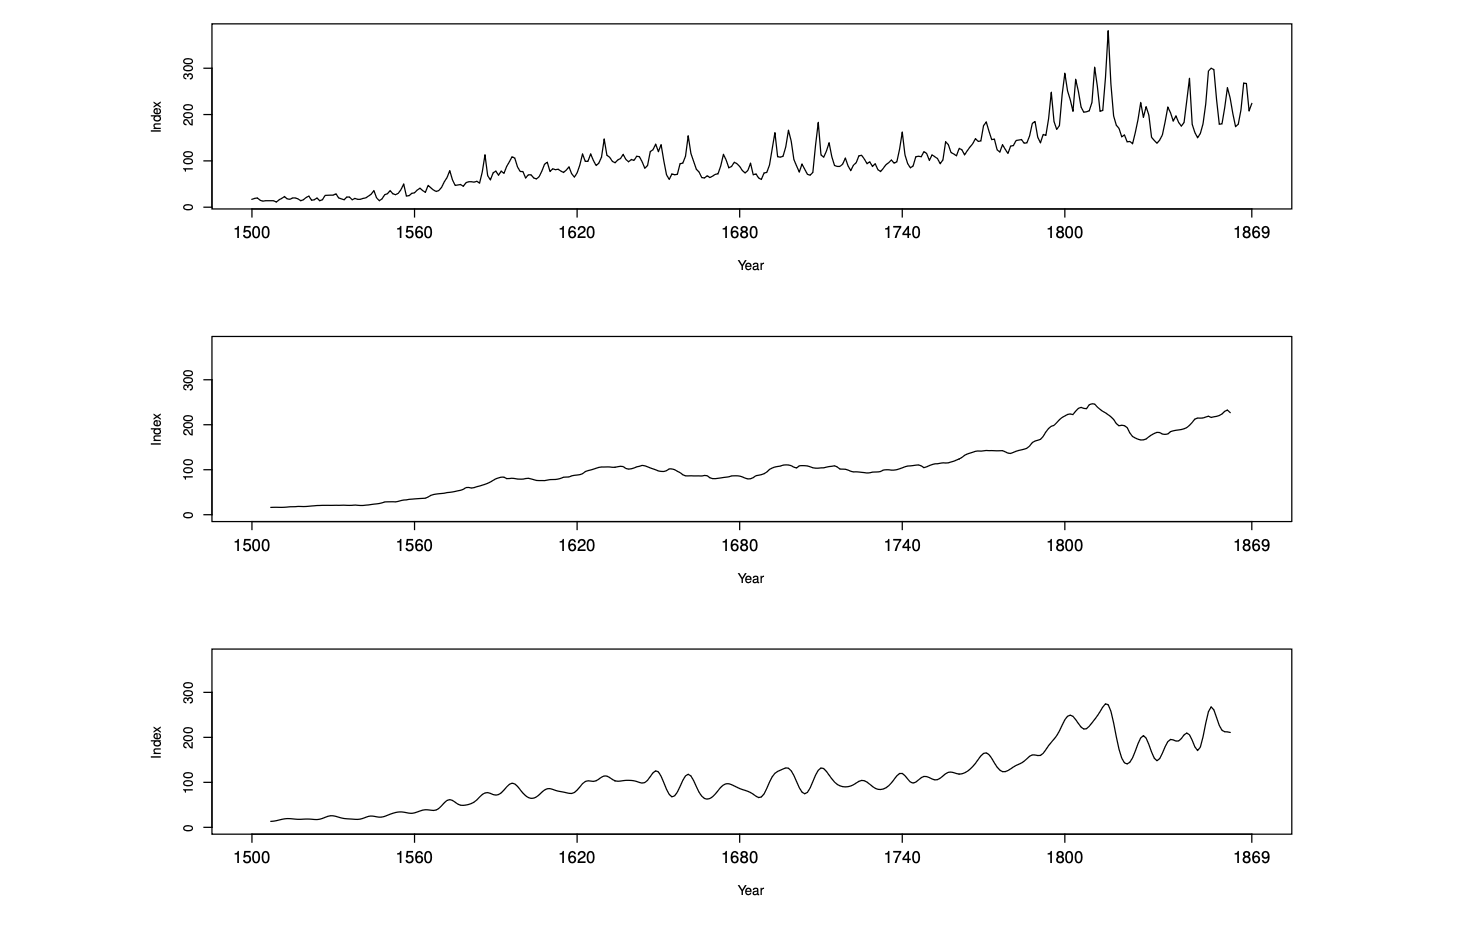
\includegraphics[width=0.8\textwidth]{Chapter 2/fig2-1.png}
	\caption{The original and smoother Beveridge wheat price annual index series from 1500 to 1869 (Top: The raw data; Middle: Smoothed series with simple moving average and $q=7$; Bottom: Smoothed series with Spencer's 15-point moving average).}
	\label{fig:2.1}
\end{figure}

The top panel of \cref{fig:2.1} shows the original time series, while the middle and bottom ones show the smoothed series via the simple moving average and Spencer's 15-point moving average.

To reproduce \cref{fig:2.1}, we can use the following piece of code:
\begin{minted}{R}
> smooth.sym<-function(my.ts, window.q){
    window.size<-2*window.q+1
    my.ts.sm<-rep(0, length(my.ts)-window.size)
    for (i in 1:length(my.ts.sm)) {
      my.ts.sm[i]<-mean(my.ts[i:(i+window.size-1)])
    }
    my.ts.sm
  } # moving average with equal and symmetric weights

> smooth.spencer<-function(my.ts){
    weight<-c(-3,-6,-5,3,21,46,67,74,67,46,21,3,-5,-6,-3)/320
    my.ts.sm<-rep(0, length(my.ts)-15)
    for (i in 1:length(my.ts.sm)) {
	  my.ts.sm[i]<-sum(my.ts[i:(i+14)]*weight)
    }
    my.ts.sm
  } # Spencer’s 15-point moving average

> library(tseries)
> data(bev)
> bev.sm<-smooth.sym(bev, 7)
> bev.spencer<-smooth.spencer(bev)
> x.pos<-c(1500, 1560, 1620, 1680, 1740, 1800, 1869)
> par(mfrow=c(3,1), mar=c(4,4,4,4))
> plot(bev, type="l", xlab="Year", ylab="Index", xaxt="n")
> axis(1, x.pos, x.pos)
> plot(c(1, length(bev)), c(0, max(bev)), type="n", xlab="Year",
ylab="Index", xaxt="n")
> lines(seq(8, length(bev)-8), bev.sm)
> axis(1, x.pos-1500+1, x.pos)
> plot(c(1, length(bev)), c(0, max(bev)), type="n", xlab="Year",
ylab="Index", xaxt="n")
> lines(seq(8, length(bev)-8), bev.spencer)
> axis(1, x.pos-1500+1, x.pos)
\end{minted}

Whenever a symmetric filter is chose, there is like to be an end-effects problem, since the symmetric filter does not take care of the end. Ideally we would want smoothened values all the way to the end of the time series, especially when doing forecasting. The analyst can project the smoothed values by eye or, alternatively, use an asymmetric filter that only involves present and past values, like exponential smoothing (Section 5.2.2):
\[ \mathrm{Sm}(x_t) = \sum_{j = 0}^{\infty} \alpha(1 - \alpha)^j x_{t-j}, \]
where $\alpha$ is a constant such that $0 < \alpha < 1$.

Having estimated the trend, we can look at the local fluctuations by examining 
\begin{align*}
	\mathrm{Res}(x_t) 
	&= \text{residual from smoothed value} \\
	&= x_t - \mathrm{Sm}(X_t) \\
	&= \sum_{r = -q}^{+s} b_rx_{t+r}.
\end{align*}
This is also a linear filter with $b_0 = 1 - a_0$, and $b_r = -a_r$ for $r \neq 0$. If $\Sigma a_r = 1$, then $\Sigma b_r = 0$ and the filter is a trend remover.

How to choose the appropriate filter? The answer to this question requires considerable experience plus knowledge of the frequency aspects of time-series analysis. Some times we may want to get rid of local fluctuations to get smoothed values (low-pass filter), while other times, we want to investigate the residuals and remove the long-term fluctuations (high-pass filter).

\textit{Filters in series}
A smoothing prodedure may be carried out in two or more stages:
\begin{figure}[h]
	\centering
	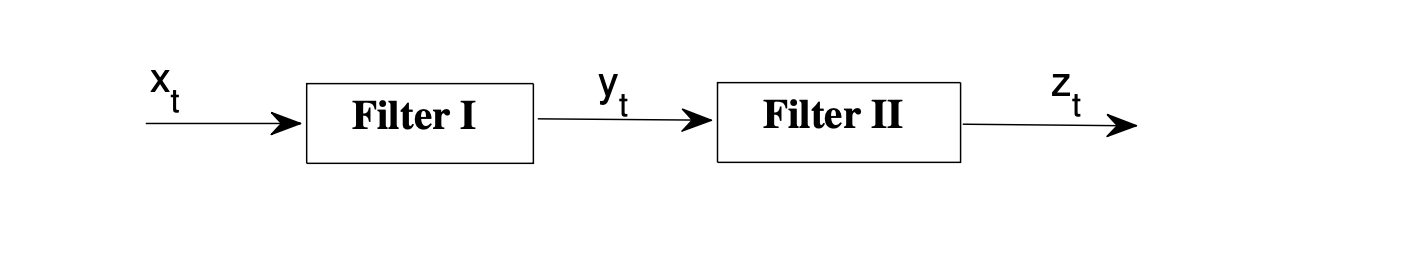
\includegraphics[width=0.8\textwidth]{Chapter 2/fig2-2.png}
	\caption{Two filters in series.}
	\label{fig:2.2}
\end{figure}

It is easy to show that a series of linear operations is still a linear filter overall. Suppose $\{ a_r \}$ are the coefficients of the first filter which gets $\{ y_t \}$ from $\{ x_t \}$, and $\{ b_j \}$ are the coefficients of the second filter which gets $\{ z_t \}$ from $\{ y_t \}$. Then 
\begin{align*}
	z_t 
	&= \sum_{j}^{} b_jy_{t+j} \\
	&= \sum_{j}^{} b_j \sum_{r}^{} a_r x_{t+j+r} \\
	&= \sum_{k}^{} c_kx_{t+k}
\end{align*}
where
\[ c_k = \sum_{r}^{} a_rb_{k-r} \]
are the weights for the overall filter. In particular, the weights $\{ c_k \}$ are obtained by a procedure called convolution, and write 
\[ \{ c_k \} = \{ a_r \} * \{ b_j \}. \]
For example, 
\[ \left( \frac{1}{4}, \frac{1}{2}, \frac{1}{4} \right) = \left( \frac{1}{2}, \frac{1}{2} \right) * 
\left( \frac{1}{2}, \frac{1}{2} \right) \]
The Spencer 15-point moving average is a convolution of four filters:
\[ \left( \frac{1}{4},\frac{1}{4},\frac{1}{4},\frac{1}{4} \right) 
* \left( \frac{1}{4},\frac{1}{4},\frac{1}{4},\frac{1}{4} \right) 
* \left( \frac{1}{5},\frac{1}{5},\frac{1}{5},\frac{1}{5}, \frac{1}{5} \right) 
* \left( -\frac{3}{4},\frac{3}{4},1,\frac{3}{4},-\frac{3}{4} \right) \]


\subsubsection{Differencing}
A special type of filtering is to take the difference of a given time series until it becomes stationary. For instance, first differencing is defined as 
\[ \nabla x_t = x_t - x_{t-1} \text{ for } t = 2, 3, \dots, N \]
while second differencing is defined as 
\[ \nabla^2 x_t = \nabla x_t - \nabla x_{t-1} = x_t - 2x_{t-1} + x_{t-2}. \]
Seasoning differences will be introduced in the next section.


\subsubsection{Other approaches}
More complicated approaches to handling trend will be mentiond later. In particular, state-space models involving trend terms will be mentioned in Chapter 10.



% ----------2.6----------
\subsection{Analyzing Series that Contain a Trend and Seasonal Variation}
Three seasonal models in common use are 
\begin{align*}
	A &\quad X_t = m_t + S_t + \varepsilon_t \\
	B &\quad X_t = m_t S_t + \varepsilon_t \\
	C &\quad X_t = m_t S_t \varepsilon_t
\end{align*}
where $m_t$ is the deseasonalized mean level at time $t$, $S_t$ is the seasonal effect at time $t$, and $\varepsilon_t$ is the random error.

Model A describes the additive case, while models B and C describe the multiplicative case. The analysis of time series, which exhibit seasonal variation, depends on whether one wants to (1) measure the seasonal effect and/or (2) eliminate seasonality.

For series that do contain a substantial trend, a more sophisticated approach is required. With monthly data, the most common way of eliminating the seasonal effect is to calculate 
\[ \mathrm{Sm}(x_t) = \frac{\frac{1}{2}x_{t-6} + x_{t-5} + \cdots + x_{t+5} + \frac{1}{2}x_{t+6}}{12}. \]

For quarterly data, the seasonal effect can be eliminated by calculating 
\[ \mathrm{Sm}(x_t) = \frac{\frac{1}{2}x_{t-2} + x_{t-1} + x_t + x_{t+1} + \frac{1}{2}x_{t+2}}{4}. \]

These smoothing procedures all effectively estimate the local (deseasonalized) level of the series. The seasonal effect itself can then be estimated by calculating $x_t - \mathrm{Sm}(x_t)$ or $x_t / \mathrm{Sm}(x_t)$ depending on whether the seasonal effect is additive or multiplicative.

As an example, \cref{fig:2.3} illustrates the decomposition of the domestic monthly sales series of Australian fortified wine by winemakers into trend, additive, seasonal, and remainder series. We can do this via the ``decompose" command in R:

\begin{minted}{R}
> wine<-read.csv("../data/aus\_wine\_sales.csv", header=F)
> wine.ts<-ts(wine[,2], frequency=4, start=c(1985,1))
# create a time series object
> wine.de<-decompose(wine.ts, type="additive")
> plot(wine.de)
\end{minted}

\begin{figure}[ht]
	\centering
	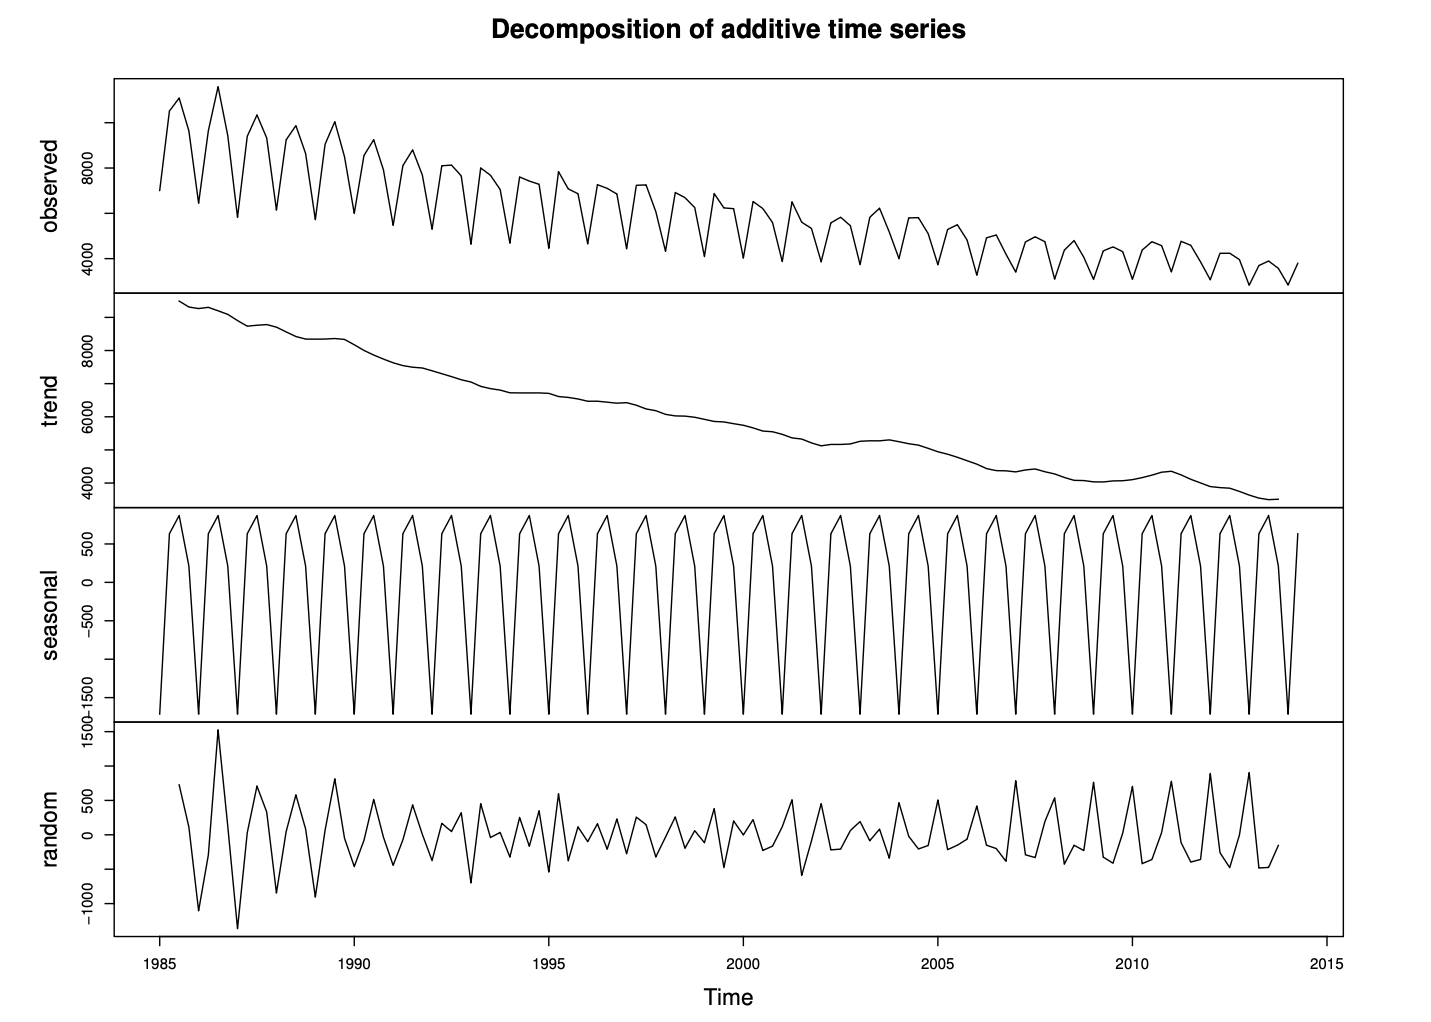
\includegraphics[width=0.8\textwidth]{Chapter 2/fig2-3.png}
	\caption{The decomposition of the domestic sales of Australian fortified wine.}
	\label{fig:2.3}
\end{figure}

Another technique of eliminating seasonal effects is seasonal filtering:
\[ \nabla_{12}x_t = x_t - x_{t-12}. \]

Two general reviews of methods for seasonal adjustment are Butter and Fase (1991) and Hylleberg (1992). Currently, the most common package for removing trend and seasonal effects is called the X-12 method. It is a fairly complicated procedure that implements a series of linear filters and adopts a recursive approach. The new software for X-12 also gives more flexibility in handling outliers, and also allows the users to deal with the possible issue of calendar effects. The X-12 method is often combined with ARIMA modeling, which gives rise to the package X-12-ARIMA. Some other countries use SEATS (Signal Extraction in ARIMA Time Series) or TRAMO (Time-series Regression with ARIMA Noise).



% ----------2.7----------
\subsection{Autocorrelation and the Correlogram}
Let's first review on the regular correlation coefficient. Given $N$ pairs of variables $x$ and $y$, say $\{ (x_1,y_1), \dots, (x_N,y_N) \}$, the sample correlation coefficient is given by 
\[ r = \frac{\sum_{i = 1}^{N} (x_i - \bar{x})(y_i - \bar{y})}{\sqrt{\sum_{i = 1}^{N} (x_i - \bar{x})^2 
\sum_{i = 1}^{N} (y_i - \bar{y})^2}}. \]
This value lies in $[-1, 1]$ and measures the strength of linear association between the two variables. 

Now, given $N$ observations $x_1, \dots, x_N$ of a time series, we can form $N - 1$ pairs of observation by getting $\{ (x_1, x_2), \dots, (x_{N-1}, x_N) \}$, where each pair of observations is seperated by 1 time interval. Then we can get a sample correlation coefficient 
\[ r_1 = \frac{
\sum_{t = 1}^{N - 1} (x_t - \bar{x}_{(1)}) (x_{t+1} - \bar{x}_{(2)})
}{\sqrt{\sum_{t = 1}^{N - 1} (x_t - \bar{x}_{(1)})^2} \sum_{i = 1}^{N - 1} (x_{t+1} - \bar{x}_{(2)})^2}, \]
where 
\[ \bar{x}_{(1)} = \frac{1}{N - 1}\sum_{t = 1}^{N - 1} x_t \]
is the mean of the first $N - 1$ observations, while 
\[ \bar{x}_{(2)} = \frac{2}{N}\sum_{t = 1}^{N - 1} x_t \]
is the mean of the last $N - 1$ observations. The quantity above is called the sample autocorrelation coefficient or a serial correlation coefficient at lag one.

However, the formula is rather complicated, so instead we can estimate using 
\[ r_1 = \frac{
\sum_{t = 1}^{N - 1} (x_t - \bar{x}) (x_{t+1} - \bar{x})
}{(N - 1)\sum_{t = 1}^{N - 1} (x_t - \bar{x})^2 / N} \]
where $\bar{x}$ is just the overall mean. We can also simplify by dropping the factor $N/(N-1)$, which is close to one if $N$ is large. This gives the even simpler formula 
\[ r_1 = \frac{
\sum_{t = 1}^{N - 1} (x_t - \bar{x}) (x_{t+1} - \bar{x})
}{\sum_{t = 1}^{N} (x_t - \bar{x})^2} \quad (*) \]
which is the form that will be used in this book.

In a similar way, we can find the correlation between observations of lag $k$, meaning 
\[ r_k = \frac{
\sum_{t = 1}^{N - k} (x_t - \bar{x}) (x_{t+k} - \bar{x})
}{\sum_{t = 1}^{N} (x_t - \bar{x})^2}. \]

In practice, the autocorrelation coefficients are calculated from the autocovariance coefficients, $\{ c_k \}$, which we define by analogy using the usual covariance formula:
\[ c_k = \frac{1}{N}\sum_{t = 1}^{N - k} (x_t - \bar{x})(x_{t+k} - \bar{x}). \]
We then compute 
\[ r_k = c_k / c_0, \ k = 0, 1, \dots, M, \text{ where } M < N. \]

Some authors use this equation instead (NOT used in this book!):
\[ c_k = \frac{1}{N - k}\sum_{t = 1}^{N - k} (x_t - \bar{x})(x_{t+k} - \bar{x}). \]


\subsubsection{The correlogram}
A useful aid in interpreting a set of autocorrelation coefficients it the correlogram. It contains the sample correlation coefficients $r_k$ for $k = 0, 1, \dots, M$ for some $M$ which is usually much less than $N$. For example, if $N = 200$ then we can use $M = 30$. Examples are shown below, from \cref{fig:2.4} to\cref{fig:2.8}.


\subsubsection{Interpreting the correlogram}
Interpreting the coefficients from the correlogram is not easy. Here are some situations:

\textit{Random series}

A time series is said to be completely random (i.i.d.) if it consists of a series of independent observations having the same distribution. For large $N$, we would expect that $r_k \approx 0$ for all $k \neq 0$. In fact, later we will see that, for a random time series, $r_k, k \geq 1$ is approximately $N(0, 1/N)$. Thus, if a time series, is random, we can expect 19 out of 20 of the values of $r_k$ to lie between $\pm 1.96/ \sqrt{N}$. As a result, it is common to regard any values of $r_k$ outside of this range to be statistically significant. This also means that even if the time series is completely random, we can find statistically significant values of $r_k$, which is a type I error.

\cref{fig:2.4} can be reproduced using the following R code:
\begin{minted}{R}
> set.seed(1)
> x<-rnorm(400)
> par(mfrow=c(2,1), mar=c(3,4,3,4))
> plot(x, type="l", xlab="", ylab="")
> title(xlab="Time", ylab="Series", line=2, cex.lab=1.2)
> acf(x, ylab="", main="")
> title(xlab="Lag", ylab="ACF", line=2)
\end{minted}

\begin{figure}[ht]
	\centering
	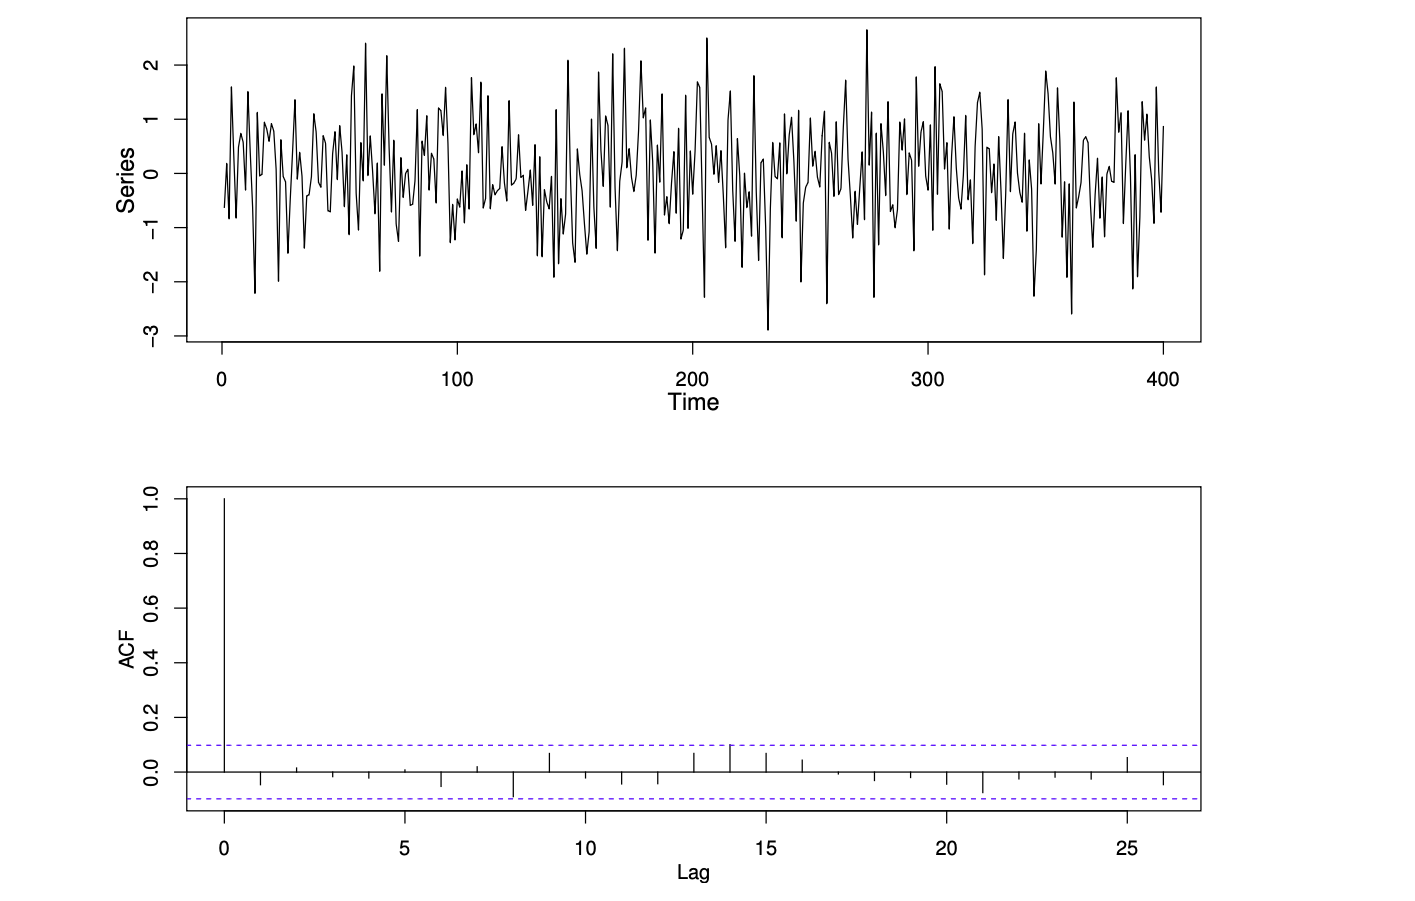
\includegraphics[width=0.7\textwidth]{Chapter 2/fig2-4.png}
	\caption{A completely random series together with its correlogram. The dotted lines in the correlogram are at $\pm 1.96 / \sqrt{N}$. Values outside these lines are said to be significantly different from zero.}
	\label{fig:2.4}
\end{figure}

\textit{Short term correlation}

Stationary series often exhibit short-term correlation characterized by a fairly large value of $r_1$ followed by one or two further coefficients that tend to decrease. Values of $r_k$ for longer lags tend to be approximately zero. An example is shown in \cref{fig:2.5}. 

\begin{figure}[ht]
	\centering
	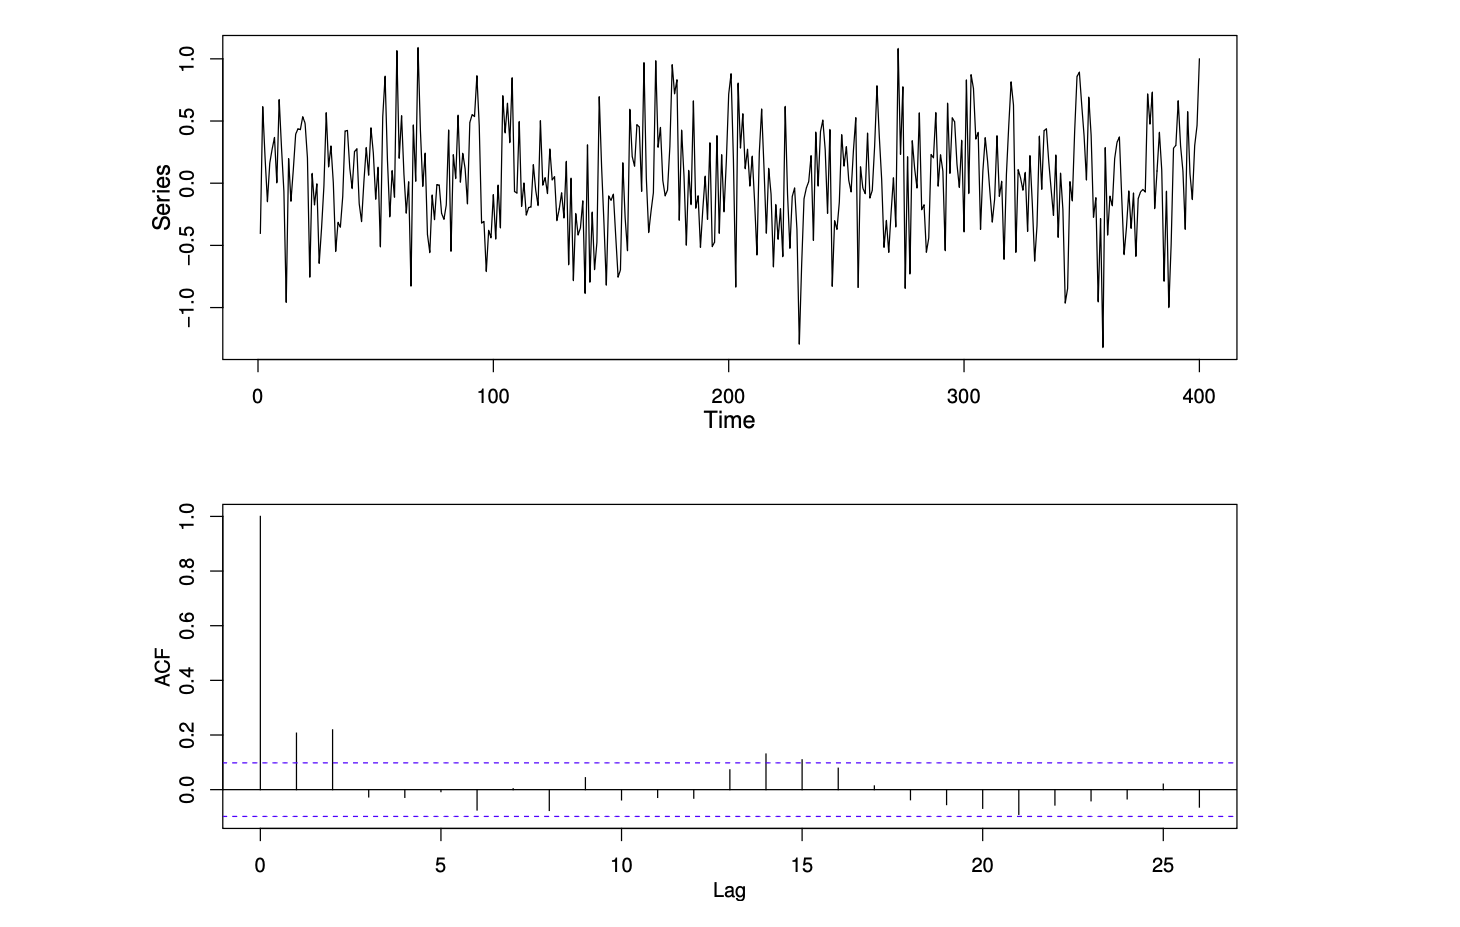
\includegraphics[width=0.7\textwidth]{Chapter 2/fig2-5.png}
	\caption{A time series showing short-term correlation together with its correlogram.}
	\label{fig:2.5}
\end{figure}

A time series that gives rise to such a correlogram is one for which an observation above the mean tends to be followed by one or more further observations above the mean, and similarly for observations below the mean.

\textit{Alternating series}

If the time series tends to alternate, so will its corrologram. An example is shown in \cref{fig:2.6}. The time series plots in \cref{fig:2.5} and \cref{fig:2.6} suggest that it is hard to distinguish between a time series with short-term correlation from that with alternating correlation. 

\begin{figure}[ht]
	\centering
	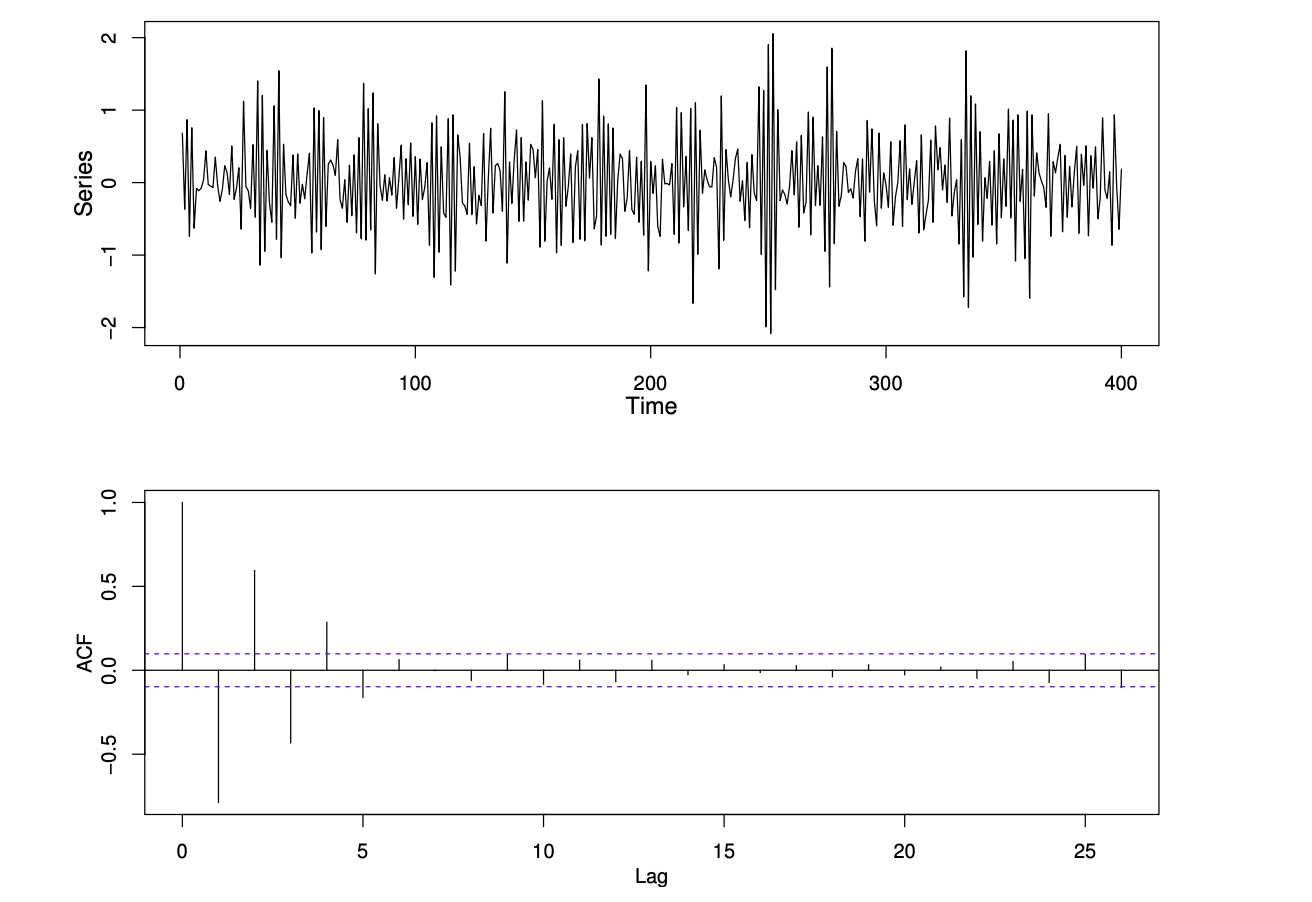
\includegraphics[width=0.7\textwidth]{Chapter 2/fig2-6.png}
	\caption{An alternating time series together with its correlogram.}
	\label{fig:2.6}
\end{figure}

\textit{Non-stationary series}
If a time series contains a trend, then the value of $r_k$ will not come down to zero except for very large values of the lag. This is because an observation on one side of the overall mean tends to be followed by a large number of further observations on the same side of the mean because of the trend. See \cref{fig:2.7} for an example. Little can be inferred from the corrologram, and any trend should be removed before calculating the set of autocorrelation coefficients $\{ r_k \}$.

\begin{figure}[ht]
	\centering
	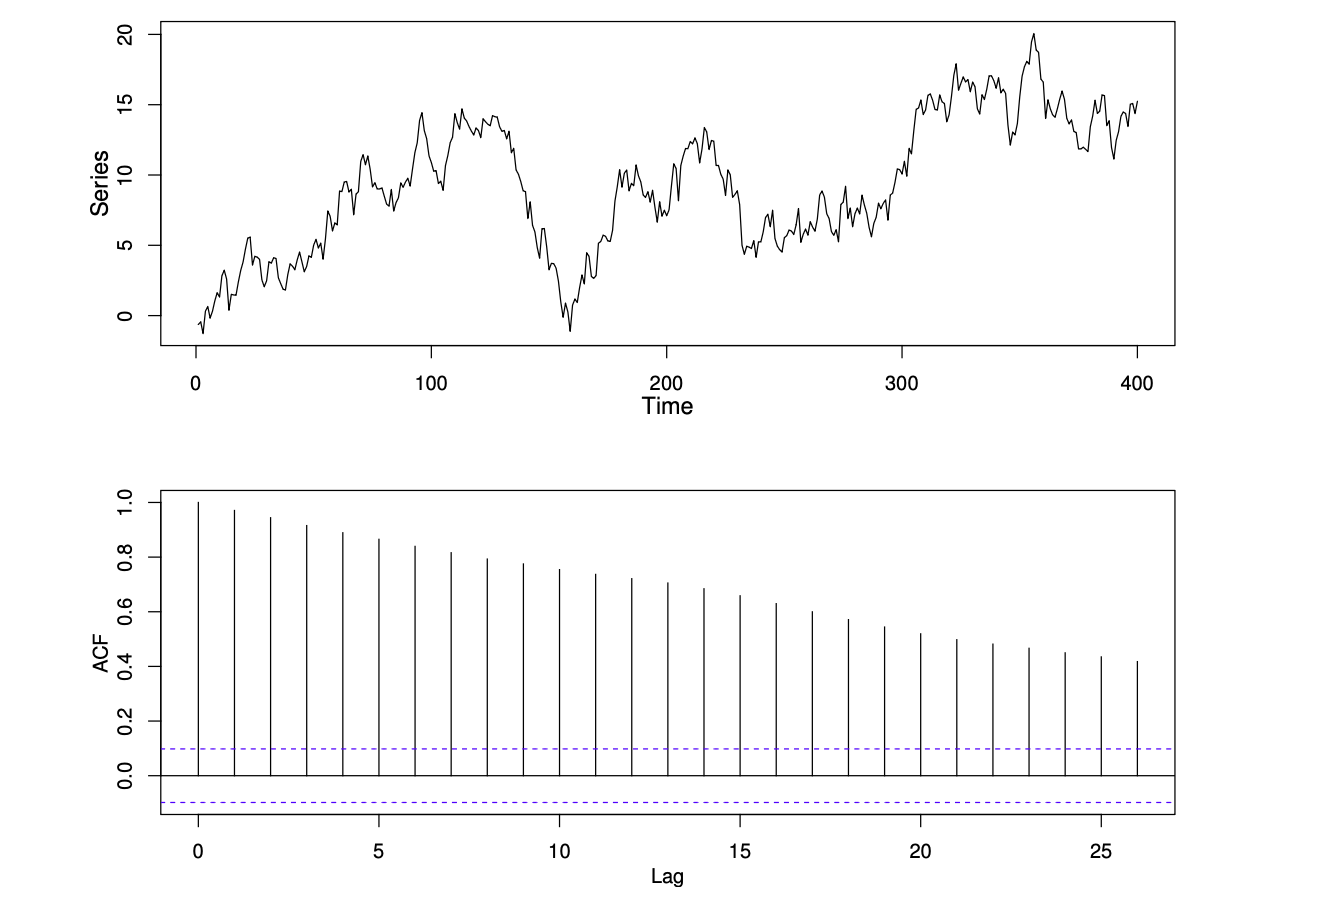
\includegraphics[width=0.7\textwidth]{Chapter 2/fig2-7.png}
	\caption{A non-stationary time series together with its correlogram.}
	\label{fig:2.7}
\end{figure}

\cref{fig:2.7} can be reproduced via the following R code:
\begin{minted}{R}
> set.seed(1)
> ts.sim3<-cumsum(rnorm(400))
> par(mfrow=c(2,1), mar=c(3,4,3,4))
> plot(ts.sim3, type="l", xlab="", ylab="")
> title(xlab="Time", ylab="Series", line=2, cex.lab=1.2)
> acf(ts.sim3, ylab="",main="")
> title(xlab="Lag", ylab="ACF", line=2)
\end{minted}

\textit{Seasonal series}
If a time series contains seeasonal variation, the corrologram will also exhibit oscillation at the same frequency. For example, with monthly observations, we expect $r_6$ to be `large' and negative, while $r_12$ will be `large' and positive. In particular, if $x_t$ follows a sinusoidal pattern, so does $r_k$. For example, if 
\[ x_t = a \cos{t \omega} \]
where $a$ is a constant and the frequency $\omega$ is such that $0 < \omega < \pi$, then it can be shown (Exercise 2.3) that 
\[ r_k \approxeq \cos{k \omega} \text{ for large } N. \]
See \cref{fig:2.8} for the corrologram of the monthly air temperature data shown in \cref{fig:1.3}.

\begin{figure}[ht]
	\centering
	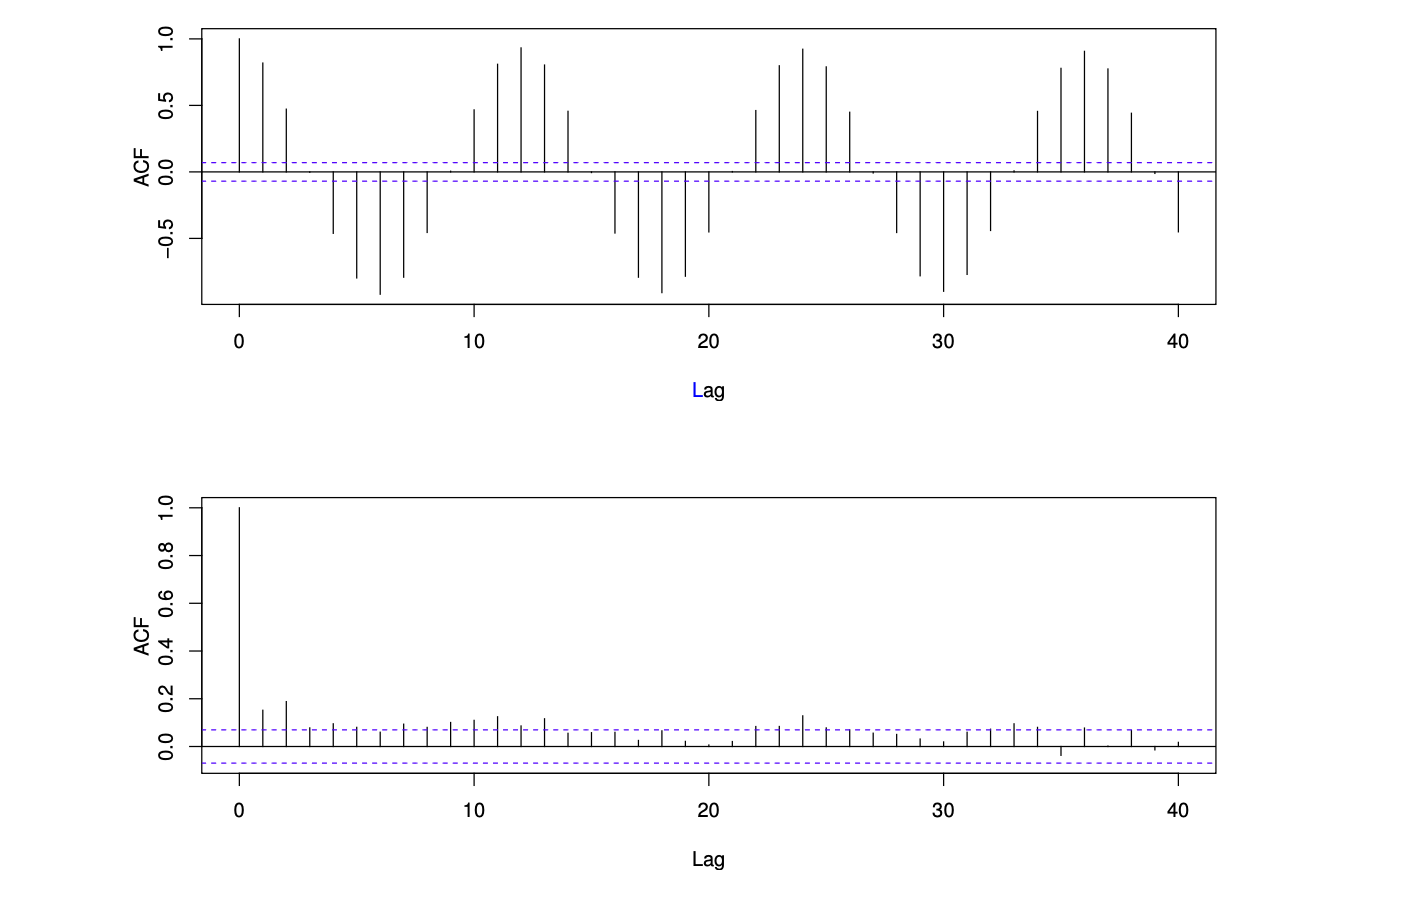
\includegraphics[width=0.8\textwidth]{Chapter 2/fig2-8.png}
	\caption{The correlograms of monthly observations on air temperature in Anchorage, Alaska for the raw data (top) and for the seasonally adjusted data (bottom).}
	\label{fig:2.8}
\end{figure}

The sinusoidal pattern of the correlogram is clearly evident, but for seasonal data of this type the correlogram provides little extra information, because the seasonal pattern is already apparent in the data. 

If the seasonal variation is removed from seasonal data, then the correlogram may provide more useful information. For example, after the seasonal effect is removed from \cref{fig:1.3}, the correlogram of the resulting series (bottom panel of \cref{fig:2.8}) shows that the first three coefficients are significantly differnt from zero, meaning there is short-term correlation.

\textit{Outliers}

If a a time series contains one or more outliers, the correlogram may be seriously affected and it is advisable to adjust these outliers before doing the formal analysis. For example, if there is one outlier in the time series at, say, time $t_0$, and if it is not adjusted, then the plot of $x_t$ against $x_{t+k}$ will contain two `extreme' points, namely, $(x_{t_0 - k}, x_{t_o})$ and $(x_{t_0}, x_{t_0 + k})$.

\textit{General remarks}
Considerable experience is required to interpret sample autocorrelation coefficients. In addition, we need to study the probability theory of stationary series and learn about the classes of models that may be appropriate. 



% ----------2.8----------
\subsection{Other Tests of Randomness}
In most cases, visual examination is enough to determine that the series is NOT random (there is trend/seasonality/short-term correlation). However, we can occasionally test whether the apparent stationary time series it `random'. One type of approach is to carry out the test of randomness in which we test whether the observations $x_1, \dots, x_N$ could have arisen in that order by chance. We'll mention a few such tests here. 

One type of test is based on counting the number of \textit{turning points}, meaning the number of times there is a local maximum or minimum in the time series. If the series is really random, one can work out the expected number of turning points and compare it with the observed value.

An alternative type of test is based on \textit{runs} of observations. For example, the analyst can count the number of runs where successive observations are all greater than the median or all less than the median, which may indicate short-term correlation. Or they can cout the number of runs of monotonicity, which may incidate trend.

Tests above are not covered in the book, since examining the correlogram is sufficient and simple enough. If a test is required though, the pormanteau test is mentioned in Section 4.7, which is based on testing for residuals.



% ----------2.9----------
\subsection{Handling Real Data}
We'll close on how to handle real data. When receiving the data, we can't assume that it's structured well already, hence we will have to clean the data first, for example: Modifying outliers, correcting obvious errors, and filling in (imputing) missing observations. The analyst should also deal with any other known peculiarities, such as a change in the way that a variable is defined during the course of the data collection process.

After cleaning the data, the next step for the time-series analyst is to determine whether trend and seasonality are present. If so, how shold such eefects be modelled, measured, or removed? The treatment of such effects and missing values is often more important than the analysis and modeling of the time-series data.

The context of the problem is crucial in deciding how to modify data, if at all, and how to handle trend and seasonality. Therefore it is essential to get background knowledge about the problem.

We close by giving a non-exhaustive list of possible actions, and can be adapted to the particular problem:
\begin{itemize}
	\item Do you understand the context? Have the `right' variables been measured?
	\item Have all the time series been plotted?
	\item Are there any missing values? If so, what should be done about them?
	\item Are there any outliers? If so, what should be done about them?
	\item Are there any obvious discontinuities in the data? If so, what does this mean?
	\item Does it make sense to transform any of the variables?
	\item Is trend present? If so, what should be done about it?
	\item Is seasonality present? If so, what should be done about it?
\end{itemize}

